
%(BEGIN_QUESTION)
% Copyright 2010, Tony R. Kuphaldt, released under the Creative Commons Attribution License (v 1.0)
% This means you may do almost anything with this work of mine, so long as you give me proper credit

Sketch connecting wires to allow this data acquisition (DAQ) module to measure the pressure sensed by the 4-20 mA loop-powered pressure transmitter at input channel {\tt IN 2}.  Be sure to specify the value of the resistor you add to this circuit!

\vskip 50pt

$$\includegraphics[width=15.5cm]{i04552x01.eps}$$

\underbar{file i04552}
%(END_QUESTION)





%(BEGIN_ANSWER)

Any solution placing the power supply, transmitter, and DAQ input channel \#2 in series with the proper polarities (power supply as source, transmitter and DAQ as loads) is correct:

$$\includegraphics[width=15.5cm]{i04552x02.eps}$$

Since this DAQ can input up to 5 volts DC of either polarity, there is no one ``correct'' polarity for the DAQ input.  The transmitter, however, {\it must} be wired with the correct polarity (as a load) or else it will not function.

%(END_ANSWER)





%(BEGIN_NOTES)

{\bf This question is intended for exams only and not worksheets!}.

%(END_NOTES)

